\documentclass[
  captions=tableheading,
  bibliography=totoc, 
  titepage=firstiscover,
]{scrartcl}

\usepackage{blindtext} %neuer input

\usepackage{longtable} % Tabellen über mehrere Seiten

\usepackage[utf8]{inputenc} %neuer input

\usepackage{scrhack}

\usepackage[aux]{rerunfilecheck} %Warnung falls nochmal kompiliert werden muss

\usepackage{fontspec} %Fonteinstellungen

\recalctypearea{}

\usepackage[main=ngerman]{babel} %deutsche Spracheinstellung

\usepackage{ragged2e} %neuer input

\usepackage{amsmath, nccmath}

\usepackage{amssymb} %viele mathe Symbole

\usepackage{mathtools} %Erweiterungen für amsmath


\DeclarePairedDelimiter{\abs}{\lvert}{\rvert}
\DeclarePairedDelimiter{\norm}{\lVert}{\rVert}

\DeclarePairedDelimiter{\bra}{\langle}{\rvert}
\DeclarePairedDelimiter{\ket}{\lvert}{\rangle}

\DeclarePairedDelimiterX{\braket}[2]{\langle}{\rangle}{
#1 \delimsize| #2
}

\NewDocumentCommand \dif {m}
{
\mathinner{\symup{d} #1}
}


\usepackage[
  math-style=ISO,
  bold-style=ISO,
  sans-style=italic,
  nabla=upright,
  partial=upright,
  warnings-off={
    mathtools-colon,
    mathtools-overbracket,
  },
]{unicode-math}

\setmathfont{Latin Modern Math}
\setmathfont{XITS Math}[range={scr, bfscr}]
\setmathfont{XITS Math}[range={cal, bfcal}, StylisticSet=1]


\usepackage[
  locale=DE,
  separate-uncertainty=true,
  per-mode=reciprocal,
  output-decimal-marker={,},
]{siunitx}

\usepackage[autostyle]{csquotes} %richtige Anführungszeichen

\usepackage{xfrac}

\usepackage{float}

\floatplacement{figure}{htbp}

\floatplacement{table}{htbp}

\usepackage[ %floats innerhalb einer section halten
  section,   %floats innerhalb er section halten
  below,     %unterhalb der Section aber auf der selben Seite ist ok
]{placeins}

\usepackage[
  labelfont=bf,
  font=small,
  width=0.9\textwidth,
]{caption}

\usepackage{subcaption} %subfigure, subtable, subref

\usepackage{graphicx}

\usepackage{grffile}

\usepackage{booktabs}

\usepackage{microtype} %Verbesserungen am Schriftbild

\usepackage[
backend=biber,
]{biblatex}

\addbibresource{../lit.bib}

\usepackage[ %Hyperlinks im Dokument
  german,
  unicode,
  pdfusetitle,
  pdfcreator={},
  pdfproducer={},
]{hyperref}

\usepackage{bookmark}

\usepackage[shortcuts]{extdash}

%\usepackage{warpcol}


\begin{document}
    \title{ATP Übungsblatt 9}
    \author{  
    Tobias Rücker\\
    \texorpdfstring{\href{mailto:tobias.ruecker@tu-dortmund.de}{tobias.ruecker@tu-dortmund.de}
    \and}{,} 
    Paul Störbrock\\
    \texorpdfstring{\href{mailto:paul.stoerbrock@tu-dortmund.de}{paul.stoerbrock@tu-dortmund.de}}{}
    }
\maketitle
\center{\Large Abgabegruppe: \textbf{Mittw. 10-12 Uhr}}
\thispagestyle{empty}

\newpage
\tableofcontents
\thispagestyle{empty}
\newpage

\setcounter{page}{1}

\section{Aufgabe 25}
\begin{figure}[H]
    \centering
    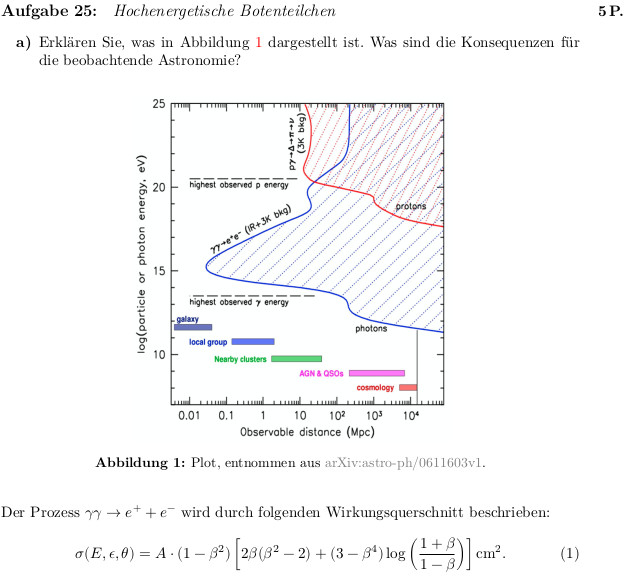
\includegraphics[width=\textwidth]{images/ex25_1.jpg}
\end{figure}
\begin{figure}[H]
    \centering
    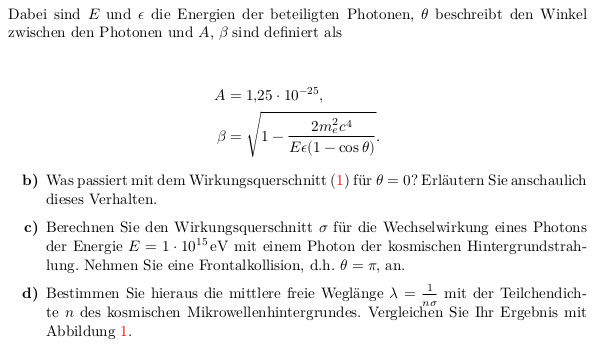
\includegraphics[width=\textwidth]{images/ex25_2.jpg}
\end{figure}


\subsection{a)}



\subsection{b)}


\subsection{c)}


\subsection{d)}



\section{Aufgabe 26}
\begin{figure}[H]
    \centering
    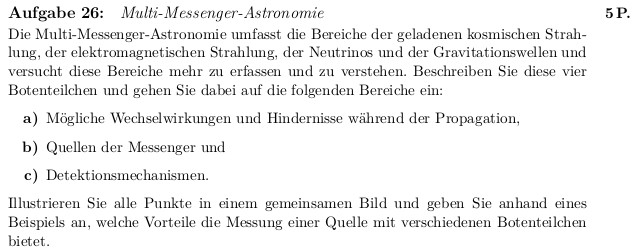
\includegraphics[width=\textwidth]{images/ex26.jpg}
\end{figure}

\subsection{a)}


\subsection{b)}


\subsection{c)}


\section{Aufgabe 27}
\begin{figure}[H]
    \centering
    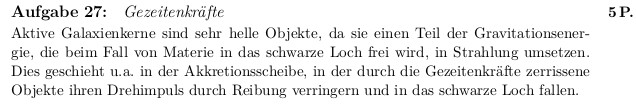
\includegraphics[width=\textwidth]{images/ex27_1.jpg}
\end{figure}
\begin{figure}[H]
    \centering
    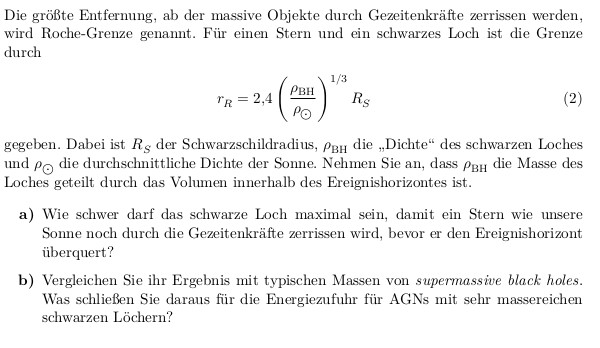
\includegraphics[width=\textwidth]{images/ex27_2.jpg}
\end{figure}



\subsection{a)}
\flushleft{Um\;}\justifying die Maximale Masse, für die die Gezeitenkräfte  massive Objekte vor Überschreitung des Erwartungshorizonts
zerreißen, zu bestimmen, wird die Formel (2) am Radius des Erwartungshorizont untersucht.
\begin{align}
    R_S &= 2,4 \left( \frac{\rho _{BH}}{\rho _{\odot}} \right)^{\frac{1}{3}} R_S \\
    \rho _{BH} &= \frac{M_{BH}}{V_{BH}} = \frac{M_{BH}4}{3 \pi R_S^3}\\
    \intertext{
        Der Schwarzschildradius berechnet bei einem stationären schwarzen Loch durch
    }
    R_S &= \frac{2GM_{HB}}{c^2}\\
    \rho_{BH} &= \frac{ c^6}{6 \pi G^3 M_{HB}^2} \\
    \intertext{weiter mit der Hauptrechnung}
    1 &= (2,4)^3 \left( \frac{c^6}{6 \pi G^3 M_{HB}^2 \rho _{\odot}} \right)\\
    M_{HB} &= \sqrt{ \frac{549 c^6}{500 \pi G^3 \rho _{\odot} } }\\
    M_{HB} &= \text{\input{M_BH.tex}}
    \intertext{
        Damit ergibt sich eine Obergrenze für die Masse von
    }
    M_{BH} \leq  \text{\input{M_BH.tex}}, \label{eq:8}
\end{align}
damit die Gezeitenkräfte vor Übertretung des Ereignishorizonts die Masse zerreißen.

\subsection{b)}
\flushleft{Typische\;}\justifying Massen von supermassiven schwarzen Löchern liegen in Größenordnungen von
$10^5\-- 10^{10} M_{\odot} $. Bei schwarzen Löchern, die in die Grenze nach Gleichung
\eqref{eq:8} fallen, wird die Energie außerhalb des Ereignishorizonts frei und
landet nicht zwangsweise im schwarzen Loch. Bei schwarzen Löchern mit höheren Massen
findet die Zerreißung erst innerhalb des Erwartungshorizonts statt und die gesamte Energie
bleibt im schwarzen Loch. Dadurch würde ein Stern wie unsere Sonne keinen Beitrag zur 
Akkretionsscheibe liefern.



\end{document}
